\documentclass{beamer}

\mode<presentation> {

%\usetheme{default}
%\usetheme{AnnArbor}
%\usetheme{Antibes}
%\usetheme{Bergen}
%\usetheme{Berkeley}
%\usetheme{Berlin}
%\usetheme{Boadilla}
%\usetheme{CambridgeUS}
%\usetheme{Copenhagen}
%\usetheme{Darmstadt}
%\usetheme{Dresden}
%\usetheme{Frankfurt}
%\usetheme{Goettingen}
%\usetheme{Hannover}
%\usetheme{Ilmenau}
%\usetheme{JuanLesPins}
%\usetheme{Luebeck}
\usetheme{Madrid}
%\usetheme{Malmoe}
%\usetheme{Marburg}
%\usetheme{Montpellier}
%\usetheme{PaloAlto}
%\usetheme{Pittsburgh}
%\usetheme{Rochester}
%\usetheme{Singapore}
%\usetheme{Szeged}
%\usetheme{Warsaw}

% As well as themes, the Beamer class has a number of color themes
% for any slide theme. Uncomment each of these in turn to see how it
% changes the colors of your current slide theme.

%\usecolortheme{albatross}
%\usecolortheme{beaver}
%\usecolortheme{beetle}
%\usecolortheme{crane}
%\usecolortheme{dolphin}
%\usecolortheme{dove}
%\usecolortheme{fly}
%\usecolortheme{lily}
%\usecolortheme{orchid}
%\usecolortheme{rose}
%\usecolortheme{seagull}
%\usecolortheme{seahorse}
%\usecolortheme{whale}
%\usecolortheme{wolverine}

%\setbeamertemplate{footline} % To remove the footer line in all slides uncomment this line
%\setbeamertemplate{footline}[page number] % To replace the footer line in all slides with a simple slide count uncomment this line

%\setbeamertemplate{navigation symbols}{} % To remove the navigation symbols from the bottom of all slides uncomment this line
}

\usepackage{graphicx} % Allows including images
\usepackage{booktabs} % Allows the use of \toprule, \midrule and \bottomrule in tables
\usepackage{listings}
\usepackage{url}
\usepackage{mathtools}

%---------------------------------------------------------------------------------------
%	TITLE PAGE
%--------------------------------------------------------------------------------------

\title[Cake Cutting]{Introduction to Decision Support based on Cake Cutting problem} % The short title appears at the bottom of every slide, the full title is only on the title page

\author{Michal Mazurek} % Your name
%\institute[UCLA] % Your institution as it will appear on the bottom of every slide, may be shorthand to save space
\date{\today} % Date, can be changed to a custom date

\begin{document}

\begin{frame}
\titlepage % Print the title page as the first slide
\end{frame}

\begin{frame}
\frametitle{Overview} % Table of contents slide, comment this block out to remove it
\tableofcontents % Throughout your presentation, if you choose to use \section{} and \subsection{} commands, these will automatically be printed on this slide as an overview of your presentation
\end{frame}

%----------------------------------------------------------------------------------------
%	PRESENTATION SLIDES
%----------------------------------------------------------------------------------------

%------------------------------------------------

\section{What is Decision Support?}

\begin{frame}
\frametitle{What is Decision Support?}
\begin{block}{The goal of Decision Support}
The main aim of decision support is proposing algorithms that simplify a process of making decisions i.e. choosing a new car, camera, etc. In other words, we look for a method which solves a specific decision problem and let us achieve a goal. 
\end{block}
\begin{block}{Decision problem}
A situation where there is a necessity to choose one of at least two possible variants of actions. A decision maker has to answer one of the following questions:
\begin{itemize}
\item How to choose the best variant? (Choice problem)
\item How to classify variants into decision classes? (Classification problem)
\item How to order variants from the best to the worst? (Ordering problem)
\end{itemize}
\end{block}
\end{frame}

\begin{frame}
\frametitle{What is Decision Support?}
\begin{center}
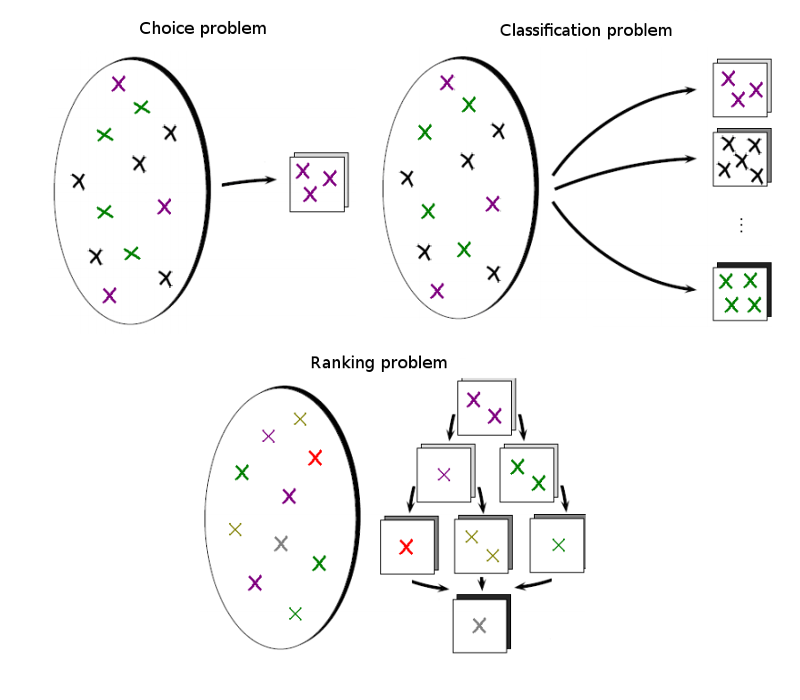
\includegraphics[scale=0.34]{problems.png}
\end{center}
\end{frame}


\subsection{Specific areas of Decision Support}
\begin{frame}
\frametitle{Specific areas of Decision Support}
\end{frame}

\subsection{What do we need to construct a decision support algorithm?}
\begin{frame}
\frametitle{What do we need to construct decision support algorithm?}
\begin{block}{Preference information}
The information that is given by decision maker in order support solving a problem.
\end{block}
\begin{block}{Preference model}
Preference model allows to aggregate evaluations on each criterion of specific variant.
It is built by preference information given by decision maker. We usually distinguish three types of preference model:
\begin{itemize}
\item function,
\item relational system,
\item set of decision rules.
\end{itemize}
\end{block}
\begin{block}{Criterion}
Criterion is a real-valued function reflecting a worth of variants from a particular point of view. Family of criteria should be consistent.
\end{block}
\end{frame}


\section{Cake cutting}
\begin{frame}
\frametitle{Cake cutting}
Cake-cutting is a metaphor for a wide range of real-world problems that involve dividing some continuous object, whether it’s cake or, say, a tract of land, among people who value its features differently. 
The ideal method, which solves the problem, should:
\begin{itemize}
\item work for any number of players,
\item make a division proportional,
\item make a division envy-free, 
\item make a division equitable. 
\end{itemize}

\end{frame}

\subsection{Historical background}
\begin{frame}
\frametitle{Historical background}
\end{frame}


\subsection{The model}
\begin{frame}
\frametitle{The model}
    Let us denote a set of players by $N={1,\dots,n}$ and our devisible good - the cake - by the interval $[0,1]$. Moreover we assume that each player is endowed with a valuation function $V_{i}$ (information preference), which maps a given subinterval $I\subseteq[0,1]$ to it by player $i$, $V_{i}(I)$. 

    We are certainly interested in allocations $A=(A_1,\dots,A_n)$, where each $A_i$ is the piece of cake allocated to agent $i$. Now we can express our criteria in a more formal way:
\begin{itemize}
    \item Proportionality: for all $i\epsilon{N}$, $V_{i}(A_i)\geq\frac{1}{n}$,
    \item Envy-freeness: for all $i,j\epsilon{N}$, $V_{i}(A_i)\geq{V_i}(A_j)$,
    \item Equitability: for all $i,j\epsilon{N}$, $V_{i}(A_i)={V_j}(A_j)$
\end{itemize}
\end{frame}


\subsection{Proportionality for n = 2: Cut and Choose}
\begin{frame}
\frametitle{Proportionality for n = 2: Cut and Choose}
\begin{enumerate}
    \item Player 1 cuts the cake into two equally-valued pieces $X_1$ and $X_2$, such that $V_1(X_1)=V_1(X_2)=\frac{1}{2}$
    \item Player 2 chooses its preferred piece and player 1 receives the remaining piece.
\end{enumerate}
\end{frame}

\subsection{Proportionality for any n: Banach-Knaster}
\begin{frame}
\frametitle{Proportionality for any n: Banach-Knaster}

\end{frame}

\subsection{Proportionality for any n: Dubins-Spanier}
\begin{frame}
\frametitle{Proportionality for any n: Dubins-Spanier}
\begin{enumerate}
    \item In the first step each player $i\epsilon{N}$ makes a mark at the point $x_i$ such that $V_{i}([0,x_i])=\frac{1}{n}$. The player $j$ that made leftmost mark exits with the piece $A_j=[0, x_j]$.
    \item If there is only one player left, it receives uclaimed piece of cake else go to step 1.
\end{enumerate}
\end{frame}

\subsection{Proportionality for any n: Even-Paz}
\begin{frame}
\frametitle{Proportionality for any n: Even-Paz}
\begin{enumerate}
    \item In the first step each player $i\epsilon{N}$ makes a mark at the point $x_i$ such that $V_{i}([0,x_i])=\frac{1}{n}$. The player $j$ that made leftmost mark exits with the piece $A_j=[0, x_j]$.
    \item If there is only one player left, it receives uclaimed piece of cake else go to step 1.
\end{enumerate}

\end{frame}


\subsection{Envy-freeness for n = 3: Selfridge-Conway}
\begin{frame}
\frametitle{Envy-freeness for n = 3: Selfridge-Conway}
\begin{table}
\begin{tabular}{c|c|c|c|}
Number of players & Proportionality & Envy-freeness & Complexity \\
\hline 
2 & yes & yes & 2 \\
\end{tabular}
\end{table}

\end{frame}

\subsection{How about an envy-free algorithm for any number of players?}
\begin{frame}
\frametitle{How about an env-free algorithm for any number of players?}
\end{frame}

%------------------------------------------------

\section{References}
\begin{frame}
\frametitle{References}
\footnotesize{
\begin{thebibliography}{99} % Beamer does not support BibTeX so references must be inserted manually as below
\bibitem[Meyers, 2002]{p1} Scott Meyers (2002)
\newblock Effective C++: 50 Specific Ways to Improve Your Programs and Design
\bibitem {p2} C++ reference
\newblock \url{http://en.cppreference.com/}
\end{thebibliography}
}
\end{frame}

%------------------------------------------------

\begin{frame}
\Huge{\centerline{The End}}
\end{frame}

%----------------------------------------------------------------------------------------

\end{document}
